\documentclass[11pt]{amsart}
\usepackage[utf8]{inputenc}
\usepackage{amssymb,amsthm,amsmath,amsfonts,mathtools,latexsym}
\usepackage{tikz}
\usetikzlibrary{arrows}

\begin{document}

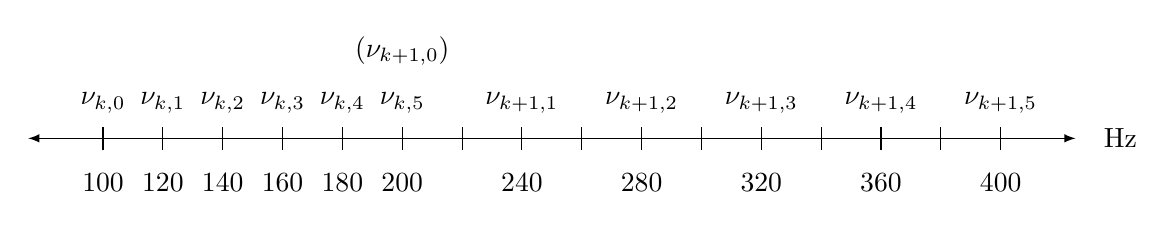
\begin{tikzpicture}[xscale = 0.19]

% draw axis
\draw [latex-latex] (-35,0) -- (35,0);
\draw (-30,-0.15) -- (-30,0.15);
\draw (-26,-0.15) -- (-26,0.15);
\draw (-22,-0.15) -- (-22,0.15);
\draw (-18,-0.15) -- (-18,0.15);
\draw (-14,-0.15) -- (-14,0.15);
\draw (-10,-0.15) -- (-10,0.15);
\draw (-6,-0.15) -- (-6,0.15);
\draw (-2,-0.15) -- (-2,0.15);
\draw (2,-0.15) -- (2,0.15);
\draw (6,-0.15) -- (6,0.15);
\draw (10,-0.15) -- (10,0.15);
\draw (14,-0.15) -- (14,0.15);
\draw (18,-0.15) -- (18,0.15);
\draw (22,-0.15) -- (22,0.15);
\draw (26,-0.15) -- (26,0.15);
\draw (30,-0.15) -- (30,0.15);

% draw labels
\node [above] at (-30,0.2) {$\nu_{k,0}$};
\node [above] at (-26,0.2) {$\nu_{k,1}$};
\node [above] at (-22,0.2) {$\nu_{k,2}$};
\node [above] at (-18,0.2) {$\nu_{k,3}$};
\node [above] at (-14,0.2) {$\nu_{k,4}$};
\node [above] at (-10,0.2) {$\nu_{k,5}$};
\node [above] at (-10,0.8) {$(\nu_{k+1,0})$};
\node [above] at (-2,0.2) {$\nu_{k+1,1}$};
\node [above] at (6,0.2) {$\nu_{k+1,2}$};
\node [above] at (14,0.2) {$\nu_{k+1,3}$};
\node [above] at (22,0.2) {$\nu_{k+1,4}$};
\node [above] at (30,0.2) {$\nu_{k+1,5}$};
\node [below] at (-30,-0.32) {$100$};
\node [below] at (-26,-0.32) {$120$};        
\node [below] at (-22,-0.32) {$140$};
\node [below] at (-18,-0.32) {$160$};
\node [below] at (-14,-0.32) {$180$};
\node [below] at (-10,-0.32) {$200$};
\node [below] at (-2,-0.32) {$240$};
\node [below] at (6,-0.32) {$280$};        
\node [below] at (14,-0.32) {$320$};
\node [below] at (22,-0.32) {$360$};
\node [below] at (30,-0.32) {$400$};

\node at (38,0.01) {Hz};

\end{tikzpicture}

\end{document}